%HW07.tex
%Seventh Homework -- Math 221H
% 
%
% Frank Sottile
% 1 October 2023 
%
%%%%%%%%%%%%%%%%%%%%%%%%%%%%%%%%%%%%%%%%%%%%%%%%%%%%%%%%
\documentclass[12pt]{article}
\usepackage{amssymb,amsmath}
\usepackage{graphicx}
\usepackage[usenames,dvipsnames,svgnames,table]{xcolor}
\usepackage{multirow}   % This is for more control over tables
%%%%%%%%%%%%%%%%%%%%%%%%%%%%%%%%  Layout     %%%%%%%%%%%%%%%%%%%%%%%%%%%%%%%%%%%%%%
\usepackage{vmargin}
\setpapersize{USletter}
\setmargrb{1cm}{0.25cm}{1cm}{0.5cm} % --- sets all four margins LTRB

%%%%%%%%%%%%%%%%%%%%%%%%%%%%%%%%%%%%%%%%  Macros  %%%%%%%%%%%%%%%%%%%%%%%%%%%%%%%%%%%%%%%%
\newcommand{\RR}{{\mathbb R}}  % This is the backboard bold symbol for the real numbers.  Note how it is used below
\newcommand{\NN}{{\mathbb N}}  % 
\newcommand{\ZZ}{{\mathbb Z}}  %

\newcommand{\calP}{{\mathcal P}}  %Caligraphic P for power set

\newcommand{\bfa}{{\bf a}}    %Vectors
\newcommand{\bfb}{{\bf b}}    %Vectors
\newcommand{\bfi}{{\bf i}}    %Unit Vectors
\newcommand{\bfj}{{\bf j}}    %Unit Vectors
\newcommand{\bfk}{{\bf k}}    %Unit Vectors

\newcommand{\sep}{{\ :\ }}     % This is for the : in our notation for building sets.
                               % an acceptable (and common) alternative is \mid  (try it!)
%%%%%%%%%%%%%%%%%%%%%%%%%%%%%%%%%%%%%%%%%%%%%%%%%%%%%%%%%%%%%%%%%%%%%%%%
\begin{document}
\LARGE 
\noindent
{\color{Maroon}Honors Multivariate Calculus \hfill Math 221H Section 201}\vspace{2pt}\\
\large
Seventh Homework:\hfill 
Due in recitation: Thursday 5 Octobr 2023\vspace{2pt}

\normalsize
    {\bf {\color{Maroon}Homework about polynomial optimization}}\vspace{2pt}

%%%%%%%%%%%%%%%%%%%%%%%%%%%%%%%%%%%%%%%%%%%%%%%%%%%%%%%%%%%%%%%%%%%%%%%%%%%%%%%%%%%%%%%%%%%%%%%%%%%%
\begin{enumerate}


%%%%%%%%%%%%%%%%%%%%%%%%%%%%%%%%%%%%%%%%%%%%%%%%%%%%%%%%%%%%%%%%%%%%%%%%%%%%%%%%%%%%%%%%%%%%%%%%%%%%
\item Find and classify all the critical points in the domains of the following functions.

  (a)\ $2x^2 + 2xy + y^2 +2x + 2y\,.$  \qquad
  (b)\  $xy+\frac{2}{x} + \frac{3}{y}\,.$  \qquad
  (c)\ $x^3+y^3-6xy\,.$
\vspace{-2pt}
%%%%%%%%%%%%%%%%%%%%%%%%%%%%%%%%%%%%%%%%%%%%%%%%%%%%%%%%%%%%%%%%%%%%%%%%%%%%%%%%%%%%%%%%%%%%%%%%%%%%

   
%%%%%%%%%%%%%%%%%%%%%%%%%%%%%%%%%%%%%%%%%%%%%%%%%%%%%%%%%%%%%%%%%%%%%%%%%%%%%%%%%%%%%%%%%%%%%%%%%%%%
\item Suppose that $f(x,y)=x^2+y^2+kxy$.
  Find and classify its critical points, and discuss how they change when $k$ takes on different values.
\vspace{-2pt}
%%%%%%%%%%%%%%%%%%%%%%%%%%%%%%%%%%%%%%%%%%%%%%%%%%%%%%%%%%%%%%%%%%%%%%%%%%%%%%%%%%%%%%%%%%%%%%%%%%%%

%%%%%%%%%%%%%%%%%%%%%%%%%%%%%%%%%%%%%%%%%%%%%%%%%%%%%%%%%%%%%%%%%%%%%%%%%%%%%%%%%%%%%%%%%%%%%%%%%%%%
\item  Find the absolute maximum and minimum points of the function $f(x,y)=x^3+3y-3xy$ over the region bounded by $y=x$, $y=0$, and $x=2$. 
\vspace{-2pt}
%%%%%%%%%%%%%%%%%%%%%%%%%%%%%%%%%%%%%%%%%%%%%%%%%%%%%%%%%%%%%%%%%%%%%%%%%%%%%%%%%%%%%%%%%%%%%%%%%%%%

   
%%%%%%%%%%%%%%%%%%%%%%%%%%%%%%%%%%%%%%%%%%%%%%%%%%%%%%%%%%%%%%%%%%%%%%%%%%%%%%%%%%%%%%%%%%%%%%%%%%%%
\item  Find the absolute maximum and minimum points of the function $f(x,y)=x^2+y^2+x^2y+4$ over the square
  $\{(x,y)\in\RR^2\mid -1\leq x,y\leq 1\}$. 
\vspace{-2pt}
%%%%%%%%%%%%%%%%%%%%%%%%%%%%%%%%%%%%%%%%%%%%%%%%%%%%%%%%%%%%%%%%%%%%%%%%%%%%%%%%%%%%%%%%%%%%%%%%%%%%

   
%%%%%%%%%%%%%%%%%%%%%%%%%%%%%%%%%%%%%%%%%%%%%%%%%%%%%%%%%%%%%%%%%%%%%%%%%%%%%%%%%%%%%%%%%%%%%%%%%%%%
\item \begin{minipage}[t]{340pt}
  A length of metal sheet 2 meters wide is to be made into a trough by bending up equal strips along both sides.
  Find the width, $x$, of the strip of metal to be bent and the angle $\phi$, so that the trough has maximum cross-sectional area.
\end{minipage}
  \qquad\begin{picture}(1,1)\put(0,-33){%
 \begin{picture}(112,33)(-1,-9)
      \put(-1,0){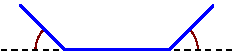
\includegraphics{images/HW07_1.eps}}
      \put(8,6){$\phi$} \put(95,6){$\phi$}
      \put(18,17){$x$} \put(88,17){$x$}  \put(50,-7){$y$}
   \end{picture}} \end{picture}
\vspace{-2pt}
%%%%%%%%%%%%%%%%%%%%%%%%%%%%%%%%%%%%%%%%%%%%%%%%%%%%%%%%%%%%%%%%%%%%%%%%%%%%%%%%%%%%%%%%%%%%%%%%%%%%

   
%%%%%%%%%%%%%%%%%%%%%%%%%%%%%%%%%%%%%%%%%%%%%%%%%%%%%%%%%%%%%%%%%%%%%%%%%%%%%%%%%%%%%%%%%%%%%%%%%%%%
\item Find the points on the surface $xy-z^2+1=0$ that are closest to the origin.
\vspace{-2pt}
%%%%%%%%%%%%%%%%%%%%%%%%%%%%%%%%%%%%%%%%%%%%%%%%%%%%%%%%%%%%%%%%%%%%%%%%%%%%%%%%%%%%%%%%%%%%%%%%%%%%

%%%%%%%%%%%%%%%%%%%%%%%%%%%%%%%%%%%%%%%%%%%%%%%%%%%%%%%%%%%%%%%%%%%%%%%%%%%%%%%%%%%%%%%%%%%%%%%%%%%%
\item Find the volume of the largest box with edges parallel to the coordinate axes that may be inscribed in the ellipsoid
  $8x^2 + 9 y^2 + 4 z^2=72$.
\vspace{-2pt}
%%%%%%%%%%%%%%%%%%%%%%%%%%%%%%%%%%%%%%%%%%%%%%%%%%%%%%%%%%%%%%%%%%%%%%%%%%%%%%%%%%%%%%%%%%%%%%%%%%%%

%%%%%%%%%%%%%%%%%%%%%%%%%%%%%%%%%%%%%%%%%%%%%%%%%%%%%%%%%%%%%%%%%%%%%%%%%%%%%%%%%%%%%%%%%%%%%%%%%%%%
\item Let $a,b,c$ be positive numbers.
  Find the  volume of the largest box in the positive octant  with three faces lying in the coordinate planes and one vertex on the plane
  $x/a+y/b+z/c=1$.    
\vspace{-2pt}
%%%%%%%%%%%%%%%%%%%%%%%%%%%%%%%%%%%%%%%%%%%%%%%%%%%%%%%%%%%%%%%%%%%%%%%%%%%%%%%%%%%%%%%%%%%%%%%%%%%%

%%%%%%%%%%%%%%%%%%%%%%%%%%%%%%%%%%%%%%%%%%%%%%%%%%%%%%%%%%%%%%%%%%%%%%%%%%%%%%%%%%%%%%%%%%%%%%%%%%%%
\item Consider the function $f(x,y)=x^3-3x^2y+y^3$.
  Show that $(0,0)$ is the only critical point of $f$, and that the discriminant test is inconclusive for $f$.

  Determine the cross-sections of $f$ obtained by considering the lines through the origin (e.g. set $y=kx$ for different values of $k$).

  What type of critical point for $f$ is the point $(0,0)$ ?
\vspace{-2pt}
%%%%%%%%%%%%%%%%%%%%%%%%%%%%%%%%%%%%%%%%%%%%%%%%%%%%%%%%%%%%%%%%%%%%%%%%%%%%%%%%%%%%%%%%%%%%%%%%%%%%

%%%%%%%%%%%%%%%%%%%%%%%%%%%%%%%%%%%%%%%%%%%%%%%%%%%%%%%%%%%%%%%%%%%%%%%%%%%%%%%%%%%%%%%%%%%%%%%%%%%%
\item At which point $(x,y)$ is the sum of the squares of the distance to the three points $(1,4)$, $(5,2)$, and $(3,2)$ minimized?

  What is the distance from this point $(x,y)$ to each of the three points?
\vspace{-2pt}
%%%%%%%%%%%%%%%%%%%%%%%%%%%%%%%%%%%%%%%%%%%%%%%%%%%%%%%%%%%%%%%%%%%%%%%%%%%%%%%%%%%%%%%%%%%%%%%%%%%%

\end{enumerate}



\end{document}
%%%%%%%%%%%%%%%%%%%%%%%%%%%%%%%%%%%%%%%%%%%%%%%%%%%%%%%%%%%%%%%%%%%
